\documentclass[crop=false, class=book]{standalone}

%pacchetto per immagini
\usepackage{graphicx}
\usepackage{subfig}

\usepackage[italian]{varioref}
\usepackage{copyrightbox}
\usepackage{url}
\usepackage{siunitx}

\begin{document}
	\chapter{Geospatial API}
	
	L'API \textit{Geospatial} è una funzionalità aggiunta a maggio 2022 al framework ARCore, che utilizza i dati di \textit{Google Earth 3D} e \textit{Google Maps Street View} per creare contenuti AR basati sulla posizione geografica. L'API sfrutta il \textit{global localization}, il quale combina il \textit{VPS - Visual Positioning Service}, un servizio Google che analizza l'ambiente circostante attraverso la fotocamera per determinare la posizione, \textit{Street View}, che fornisce un database di immagini di luoghi, e il machine learning per migliorare la determinazione della posizione del dispositivo \cite{googleblog2019global}.
	\\
	\noindent
	Il Geospatial API compara le informazioni provenienti dalla fotocamera (figura~\vref{fig:geospatial_a}) e dai sensori del dispositivo, come il GPS, con miliardi di immagini 3D estratte tramite machine learning da Street View (figura~\vref{fig:geospatial_b}) per determinare la posizione e l'orientamento del dispositivo, per poi mostrare contenuti AR posizionati correttamente rispetto all'utente, come spiegato in \cite{googleblog2022geospatial}.
	
	\begin{figure}[tbph]
		\centering
		\subfloat[][\emph{Immagini della fotocamera del dispositivo} \label{fig:geospatial_a}]
		{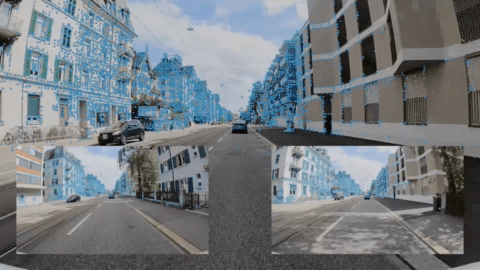
\includegraphics[width=0.47\textwidth]{./resources/images/geospatial/a.png}}  \quad
		\subfloat[][\emph{Confronto con immagini Street View} \label{fig:geospatial_b}]
		{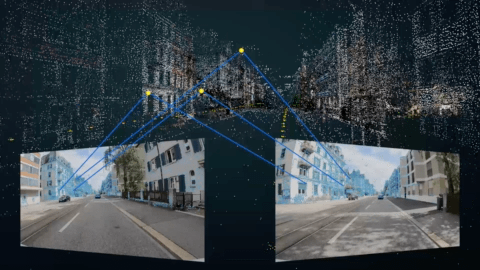
\includegraphics[width=0.47\textwidth]{./resources/images/geospatial/b.png}} \quad
		\caption{Ricostruzione delle funzionalità di Geospatial API.}
		\label{fig:geospatial}
	\end{figure}

	\section{Configurazione e utilizzo}
	La sessione ARCore deve abilitare l'utilizzo di Geospatial API, come descritto dal listing~\vref{lst:geo_session} tratto dalla documentazione ufficiale \cite{google2022geospatial}.
	
	\begin{center}
		\begin{minipage}{0.95\textwidth}
			\begin{lstlisting}[caption={Configurazione della modalità Geospatial API.}, label={lst:geo_session}, language=Kotlin]
			// Abilita il Geospatial API.
			session.configure(session.config.apply{ geospatialMode= Config.GeospatialMode.ENABLED})
			\end{lstlisting}
		\end{minipage}
	\end{center}
	
	\subsection{Configurazione di VPS}
	L'utilizzo di Visual Positioning System impone che l'app sia associata a un progetto Google Cloud Project con abilitato il ARCore API. \`E inoltre necessaria un'autenticazione tramite \textit{OAuth client}, oppure con \textit{API key}. Si veda il paragrafo~\vref{subsec:auth} del capitolo Cloud Anchor per specifiche su entrambi i tipi di autenticazione.
	\\
	Sono necessari inoltre i permessi per accedere alla posizione e ad internet per comunicare con il servizio online Geospatial API, da dichiarare nel campo \verb|manifest| del file \verb|AndroidManifest.xml|, come descritto dal listing~\vref{lst:geo_perm}.
	
	\begin{center}
		\begin{minipage}{0.95\textwidth}
			\begin{lstlisting}[caption={Richiesta di permessi per l'uso di Geospatial API.}, label={lst:geo_perm}, language=xml, morekeywords={android:name, android:value}, keywordstyle={\color{NavyBlue}\bfseries}, alsodigit={-}, stringstyle={\color{ForestGreen}\ttfamily}, emph={manifest, uses-permission},emphstyle={\color{OrangeRed}}]
			<manifest ...>
				<uses-permission android:name="android.permission.ACCESS_FINE_LOCATION"/>
				<uses-permission android:name="android.permission.ACCESS_COARSE_LOCATION"/>
				<uses-permission android:name="android.permission.INTERNET"/>
			</manifest>
			\end{lstlisting}
		\end{minipage}
	\end{center}

	\subsection{Calcolo della posizione}
	La posizione può essere presa da un oggetto della classe \verb|Earth|, ricevuto dalla sessione ARCore \verb|session|, come descritto dal listing~\vref{lst:geo_current}. Se l'oggetto di tipo \verb|Earth| ha stato \verb|TrackingState.TRACKING|, la posizione può essere ottenuta tramite un oggetto di tipo \verb|GeospatialPose|, che contiene la latitudine e la longitudine, l'altitudine e un'approssimazione della direzione verso cui il dispositivo è rivolto.
	\begin{center}
		\begin{minipage}{0.95\textwidth}
			\begin{lstlisting}[caption={Calcolo della posizione corrente.}, label={lst:geo_current}, language=Kotlin]
			val earth = session.earth
			// Verifico che sia in stato TRACKING
			if (earth?.trackingState == TrackingState.TRACKING) {
				val cameraGeospatialPose : GeospatialPose = earth.cameraGeospatialPose
				
				// Salvataggio della latitudine in gradi
				val latitude : Double = cameraGeospatialPose.latitude
				// Salvataggio della longitudine in gradi
				val longitude : Double = cameraGeospatialPose.longitude
				// Salvataggio dell'altitudine in metri
				val elevation : Double = cameraGeospatialPose.altitude
				// Salvataggio dell'orientamento in gradi
				val heading : Double = cameraGeospatialPose.heading
			}
			\end{lstlisting}
		\end{minipage}
	\end{center}
	\noindent
	L'oggetto \verb|GeospatialPose| specifica anche l'accuratezza $A$ dei dati ricevuti, tramite i metodi \verb|getHeadingAccuracy()|, \verb|getHorizontalAccuracy()| e \verb|getVerticalAccuracy()|. I valori restituiti dai metodi hanno stessa unità di misura dei valori stimati $E$ di cui specificano la precisione, cioè gradi per la latitudine, la longitudine e l'orientamento e metri per l'altitudine, e specificano che la posizione reale $R$ è compresa con una probabilità del $68\%$ nell'intervallo:
	\[
		R \in [E-A, E+A].
	\] 
	Ad esempio, se il metodo \verb|GeospatialPose.getHeading()| restituisce il valore $E = \SI{60}{\degree}$ e il metodo \verb|GeospatialPose.getHeadingAccuracy()| ritorna una precisione di $A = \SI{10}{\degree}$, il valore reale sarà con probabilità del $68\%$ nell'intervallo $R \in [\SI{50}{\degree}, \SI{70}{\degree}]$. Un valore alto di accuratezza quindi garantisce una precisione minore.

	\subsection{Posizionamento di un anchor Geospatial}
	Per il posizionamento di un anchor, i valori di latitudine e longitudine devono essere dati rispettando le specifiche WGS84, mentre l'altitudine è definita come la distanza in metri dall'elissoide definito dallo stesso standard. 
	L'orientamento dell'anchor invece viene fatto con l'utilizzo di un quaternione \verb|(qx,qy,qz,qw)|. Si veda il listing~\vref{lst:geo_pos} per un esempio di creazione dell'anchor.
	\begin{center}
		\begin{minipage}{0.95\textwidth}
			\begin{lstlisting}[caption={Posizionamento di anchor Geospatial.}, label={lst:geo_pos}, language=Kotlin]
			if (earth.trackingState == TrackingState.TRACKING) {
				val anchor = earth.createAnchor (
				/* Valori della posizione */
				latitude,longitude,altitude,
				/* Valori della rotazione */
				qx,qy,qz,qw)
				// ...
			}
			\end{lstlisting}
		\end{minipage}
	\end{center}
	\noindent
	L'altitudine dell'anchor, se esso viene posizionato vicino all'utente, può avere lo stesso valore dell'altitudine restituita dal metodo \verb|GeospatialPose.getAltitude()|. Se invece l'anchor deve avere un'altitudine diversa da quella dell'utente, essa può essere ricavata dall'API Google Maps, forzando la prospettiva 2D e convertendo il valore restituito, basato sullo standard EGM96, nella codifica WGS84.
	
	
	
	
	
	
	
	
	
	
\end{document}